%\section{Introduction}
\begin{figure}[h]
\vspace*{-0mm}
\hspace*{-6mm}
	\centering
	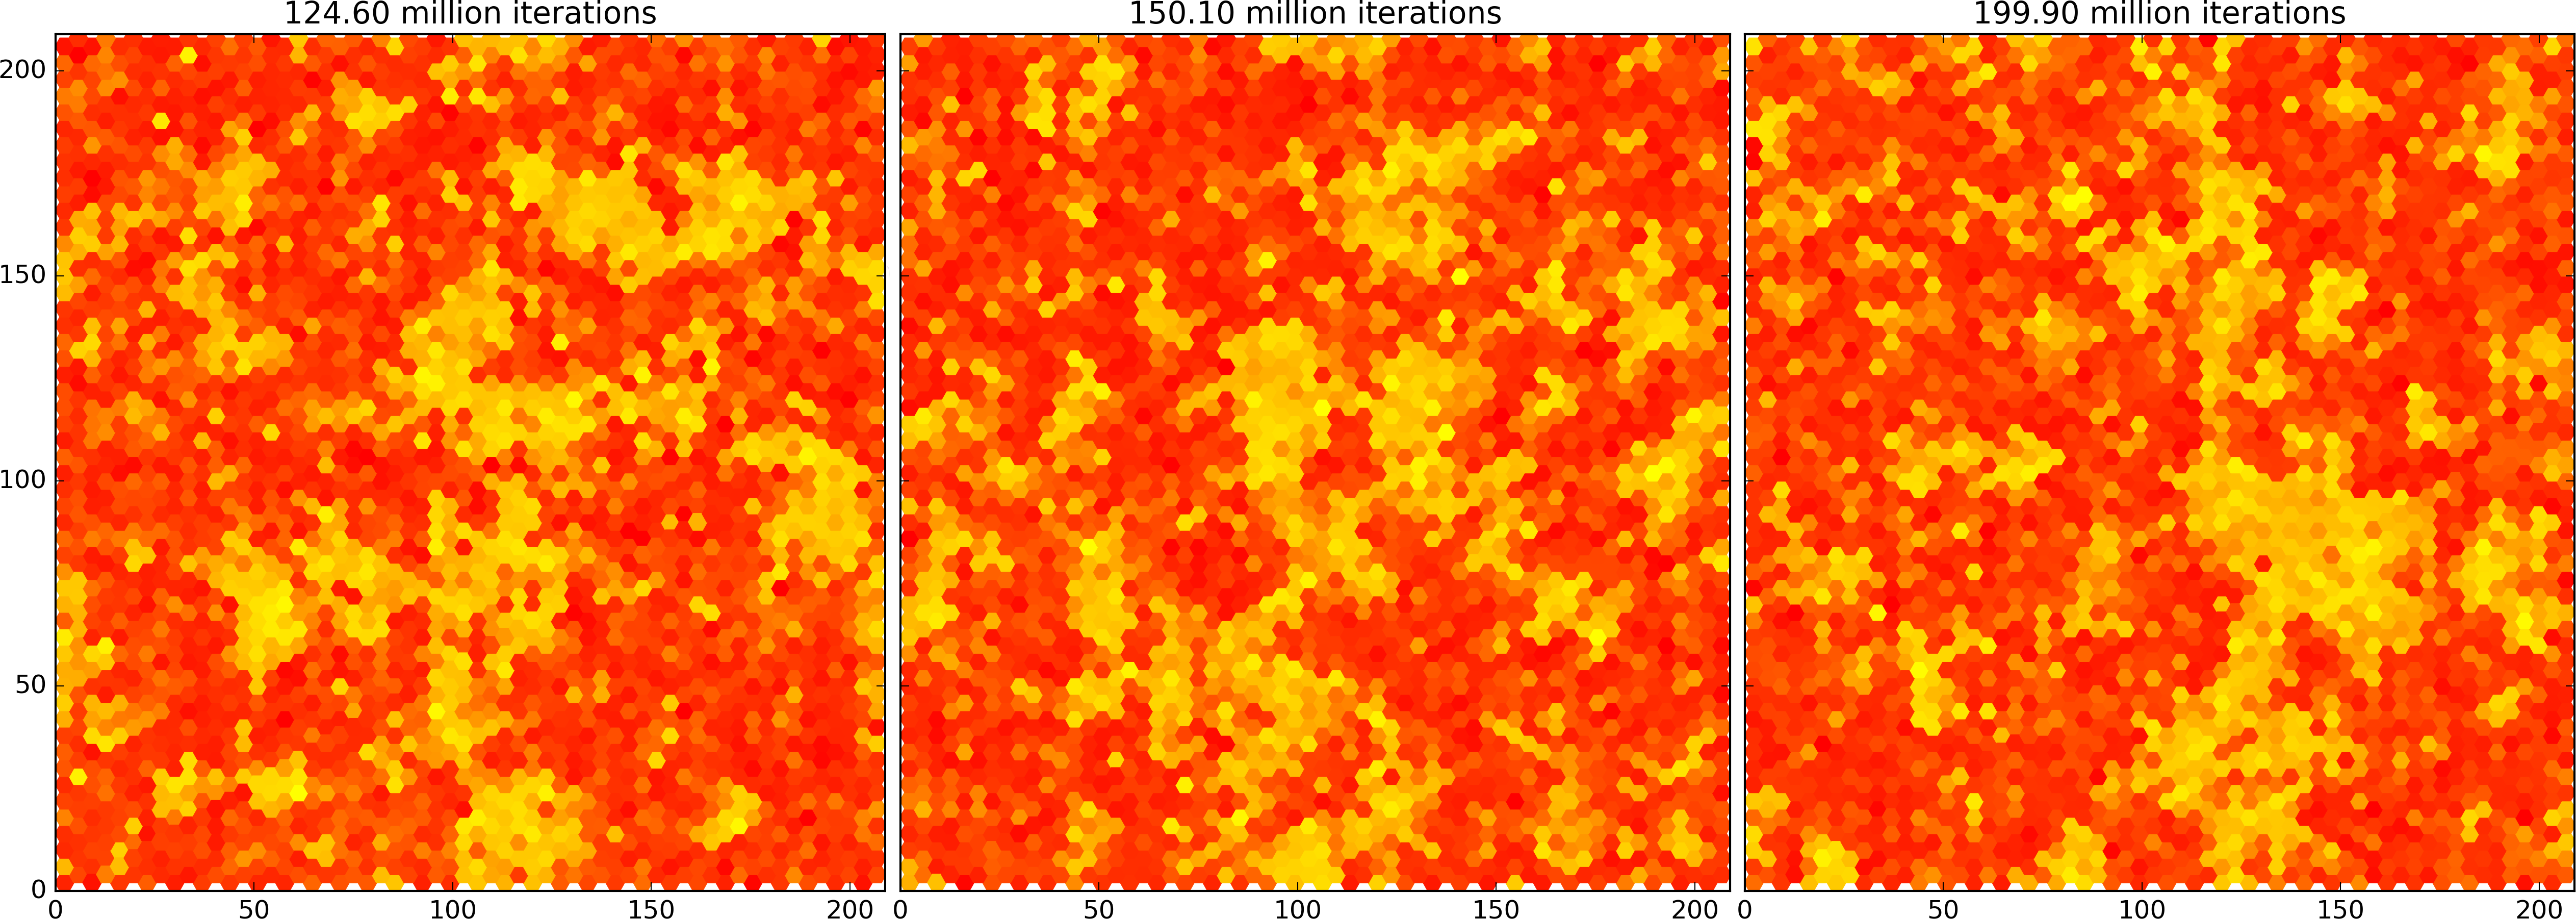
\includegraphics[width=\textwidth]{renorm}
	\caption{
	%\tiny	
	\scriptsize
	Here a simulation of a 2d fluid near the critical point is presented. The three images are the same fluid seperated in time. The interface between liquid and gas evolves in time as each globule will interact with neighboring globules. If the temperature is increased past the critical point, the globules shrink in size to the point the plots appear as white noise. Two opposing forces are at work near the critical point: entropy and energy. The universe prefers a lower energy state, and so the surface area of the liquid prefers to be minimized. Unfortunately as the temperature is increased the density of the liquid goes down while the density of the vapor goes up; which means the surface tension decreases as the temperature reaches the critical point. Near the critical point the surface tension is no longer sufficient to keep the liquid seperate from the gas, as such the liquid and gas start to mix and in the process entropy increases. 
Another way to think about the mixing is through density fluctuations. Both the liquid and gas will have density fluctuations, and as the critical point is reached the density of the gas approaches the density of the liquid, which means the density fluctuations of the gas will be enough to convert some regions into a liquid and vice versa.}
	\label{fig:renorm}
\end{figure}

The liquid-vapor phase coexistence can be found by just placing some liquid into a sealed container. Some of the liquid will evaporate into the jar creating a vapor pressure. Provided we placed enough liquid into the jar, the system will now contain both a liquid and a vapor at the same time. By sealing the liquid into a jar, we have forced the pressure of the liquid to be the same as the pressure of the gas. By allowing the atoms to swap between the liquid and gas phase, we have also allowed the chemical potential of the liquid to be the same as that of the gas.

Although we can find the phase coexistence by physically sealing a liquid in a jar, an equivalent computational method is to use an empirically determined fluid model which we can use to run simulations that also equalize the pressure and chemical potential. The problem with the computational method is the empirical model requires fitting a few parameters to data, data which probably already includes points on the phase coexistence curve. The main benefit to the computational approach is that once the empirical parameters are found, we can then create the phase coexistence of a mixture of fluids using the previously determined parameters.

One of the difficulties with the computer simulations is computation time. A simulation with a handful of atoms can be finished within 20 minutes, yet a simulation with a 100 atoms can take as long as 4 days. Further compounding the problem, to recreate the phase coexistence graph of T vs density requires setting the pressure and chemical potential of both phases equal to each other, but this is equivalent to plotting the free energy as a function of density and searching for a common cotangent. For even a simulation using a small box, the problem is plotting free energy as a function of density requires many simulations at various densities; some simulations containing only a handful of atoms while other simulations containing as much as a couple hundred atoms. Total computation time for 10 computer cores to create the free energy as a function of density graph can take as long as three weeks.

Naturally there is a tradeoff between a realistic computation time for a project and how realistic the results are going to be. The simulations use periodic boundary conditions which is just the thermodynamic way of saying the boundary should not affect the bulk properties. The key part being whatever is in the simulation is considered the bulk, which is a problem since a small simulation can hardly be considered the bulk. To get around this problem, the simulation size is usually increased until the simulation does represent the bulk. 

Normally increasing the simulation size is just fine, but there is a regime where the bulk properties depend on length scales of the order of a millimeter. This regime occurs near the critical point. As the temperature of the liquid is increased the density will naturally decrease due to thermal vibrations; conversely this increase in temperature also causes the density of the gas to increase due to the ejection of atoms at the liquid-vapor interface. As the temperature increases there is a point where the density of the liquid approaches that of the gas; this point is called the critical temperature.

Two opposing forces are at work near the critical point: entropy and energy. The universe prefers a lower energy state, and so the surface area of the liquid prefers to be minimized. Unfortunately near the critical point the density of the liquid is nearly the same as the gas; which means the surface tension decreases as the temperature reaches the critical point. This means near the critical point the surface tension is no longer sufficient to keep the liquid seperate from the gas, as such the liquid and gas start to mix and in the process entropy increases. 

Mixing near the critical point is a problem since the old idea that the thermodynamic observables are independent of the boundary conditions no longer applies. The boundary itself is now a significant contribution to the bulk properties. Unfortunately this means the simulations now need to be increased to about the same size as that of the largest fluctuation. For example, a liquid-gas system at the critical point can experience fluctuations on length scales of 1mm; a simulation with such a large box size would contain roughly $10^{19}$ atoms, which would require an unfeasible computation time.

To get around the large fluctuation problem, generalized renormalization group theory(GRG) can be applied. Simply put, GRG is a method in which fine details are omitted from calculations while still maintaining accuracy. This is done through an iterative process which incorporates interactions at progressively longer wavelengths. The zeroth order is just the ideal gas term in which all atoms only interact with the walls of the enclosure. The next order is applied via SAFT-VR in which perturbations are made to include a mean interaction and interactions up to some unknown length scale L. Longer wavelength interactions can then be applied using GRG in which the unknown length scale L is left to be found at a later time.

The main problem this project addresses is how to find the arbitrary parameter L. Usually the arbitrary parameter L is fit to experimental data. However; extra arbitrary parameters tend to reduce the predictive capability of a theory. To test whether or not the arbitrary parameter is really arbitrary, this project attempts to find the arbitrary parameter L by comparing SAFT-VR to Monte Carlo simulations. The idea is the Monte Carlo simulations using a box size with side length L should only incorporate wavelength interactions of length L, so such a simulation should give the same results as SAFT-VR. To find the paramter L, the box size of the Monte Carlo simuations and the thermodynamic variables are compared to SAFT-VR. Once an optimal box size is found, the parameter L is tested by comparing the phase coexistence of the Monte Carlo simulations to the results from SAFT-VR.